\section{BACKGROUND}
\label{sec:background}

We focus on the stochastic bandit setting in this paper where the policy or the values of the actions are represented using a 2-layers neural networks.  
However, our results can be easily generalized to many other reinforcement learning settings, e.g. state dependent stochastic bandit settings and episodic MDP settings.

\subsection{STOCHASTIC BANDIT SETTINGS}
\label{subsec:settings}

One can think of that the standard stochastic bandit setting has only 1 state.  
At each time step $t$, the agent takes an action $A_t \in [h]$ according to its own strategies $\rvpi_t$, and then it observes a random reward $R_{A_t} \in \sR$, where the mean value of $R_{A_t}$ is $r_{A_t}$. 
The agent then improves its action selection strategies. 
After such $T$ time steps, the performance of the agent's strategy is measured by the (expected) regret,
\begin{equation}
\label{eq:expected_regret}
R_n = \sum\limits_{t=0}^{T-1}{{\rvpi^*}^\top \rvr} - \sE \left[ \sum\limits_{t=0}^{T-1}{  r_{ A_t}  } \right] 
%= \sum\limits_{t=0}^{T-1}{{\rvpi^*}^\top \rvr} - \sum\limits_{t=0}^{T-1}{ \sE \left[ r_{A_t} \right] },
\end{equation}
where the expectation is over the randomness of action selection, if the agent is using some stochastic strategies.
Obviously, $\rvpi^*$ is a one-hot vector and by standard calculation, one can show that
\[
R_n = \sum_a \sum_{t=1}^T \rvpi_t(a) \Delta(a),
\]
where $\Delta(a) = \max_b r(b)- r(a)$, $r(a)$ is the expected reward of the action $a$.

%\subsubsection{Episodic Markov decision process (MDP) (maybe remove this section)}
%The episodic MDP setting recovers the bandit setting as a special case. The environment randomly select a starting state $\rvs_i^0 \in \sR^d$. At each time step $t$, the agent takes one action $A_t \in [h]$ according to some strategies, and then it observes a reward $R_{i, A_t} \in \sR$ and next state $S_{t+1} \sim \sP\left( \cdot \middle| S_t, A_t \right)$, where $\sP$ is the transition probability matrix and it is unknown to the agent. After such $H$ steps, the agent observes an ending state $S_H$, and the current trajectory terminates. At the next time step, the agent will observe a new starting state $\rvs_i^0$ randomly generated by the environment. Since we use policy gradient method (no value learning), the agent updates its NN policy weights using the cumulative reward collected after each single trajectory terminates.


\begin{figure}[t]
\vskip 0.2in
\begin{center}
\centerline{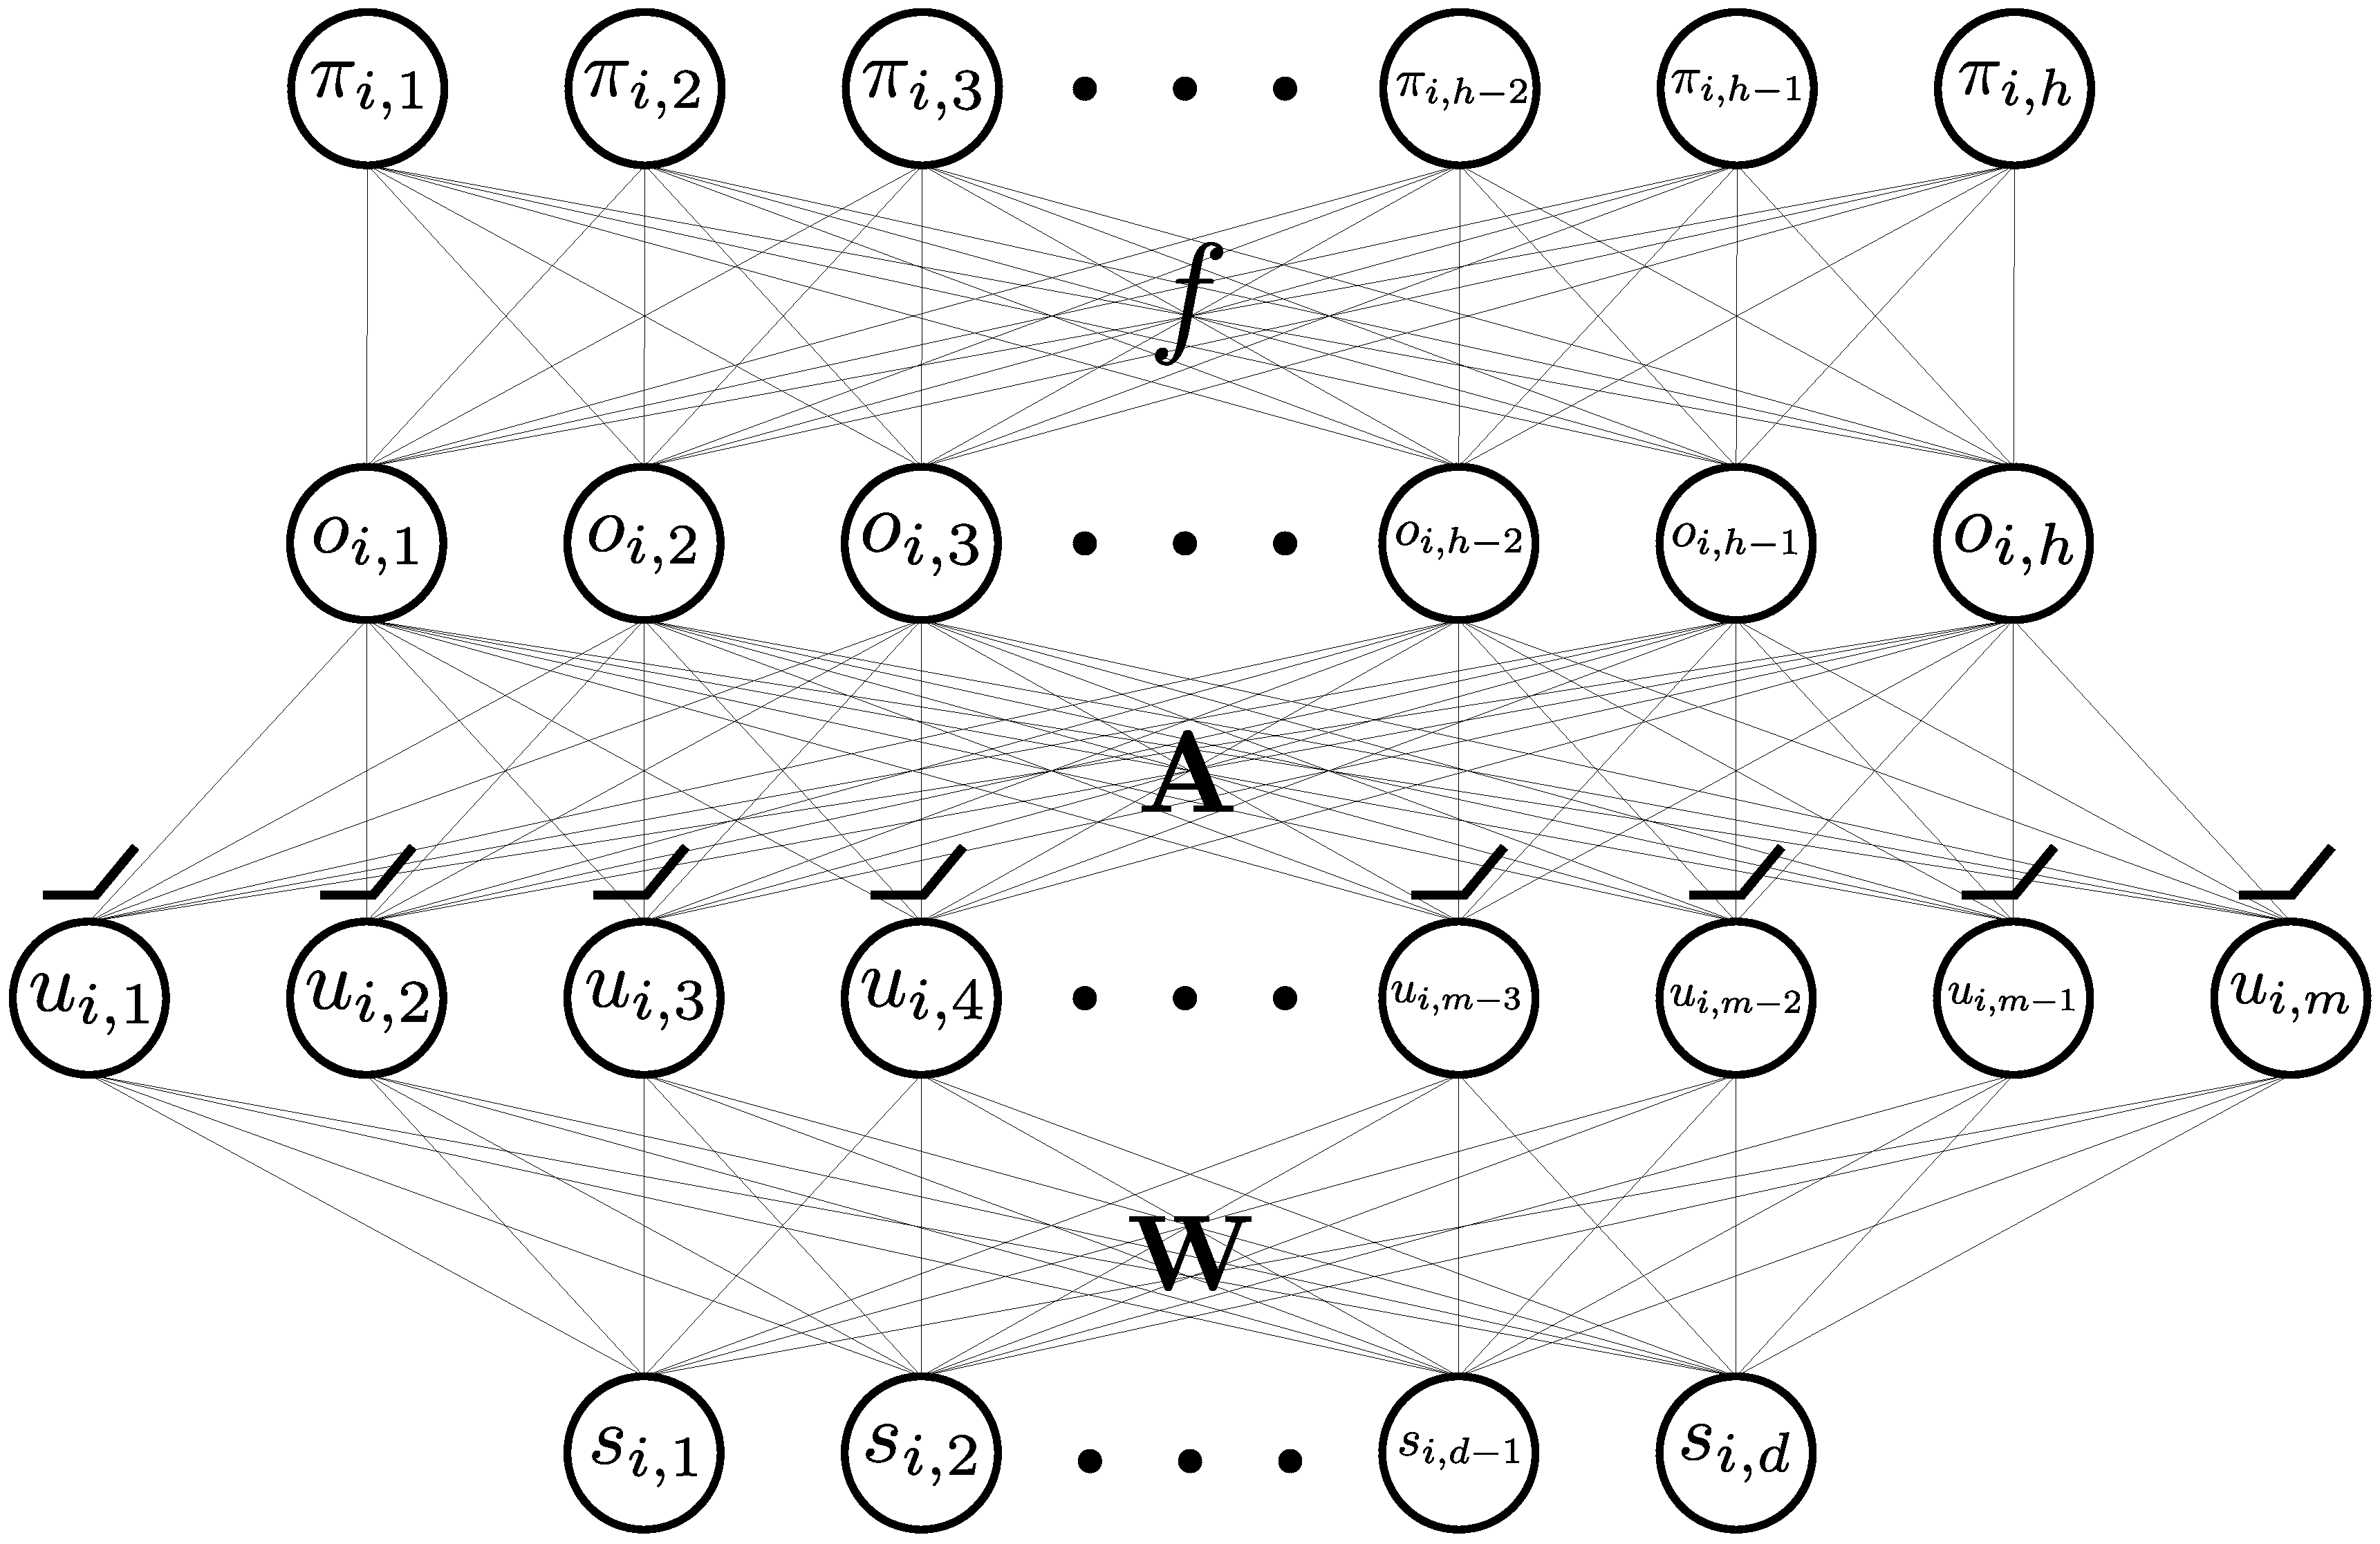
\includegraphics[width=\columnwidth]{nn_policy.pdf}}
\caption{Policy neural network.}
\label{fig:nn_policy}
\end{center}
\vskip -0.2in
\end{figure}


%We mainly focus on the standard stochastic bandit setting with $n = 1$, i.e., there is only one state $\rvs_i$. At each time step $t$, the agent takes an action $A_t \in [h]$ according to its own strategies, and then it observes a random reward $R_{i, A_t} \in \sR$, where the mean value of $R_{i, A_t}$ is $r_{i, A_t}$. The agent then uses the reward to improve its action selection strategies. After such $T$ time steps, the performance of the agent's strategy is measured by the (expected) regret,
%\begin{equation}
%\label{eq:expected_regret}
%    \sum\limits_{t=0}^{T-1}{{\rvpi_i^*}^\top \rvr_i} - \sE \left[ \sum\limits_{t=0}^{T-1}{  r_{i, A_t}  } \right] = \sum\limits_{t=0}^{T-1}{{\rvpi_i^*}^\top \rvr_i} - \sum\limits_{t=0}^{T-1}{ \sE \left[ r_{i, A_t} \right] },
%\end{equation}
%where the expectation is over the randomness of action selection, if the agent is using some stochastic strategies.


\subsection{NEURAL NETWORK VALUE FUNCTION APPROXIMATION AND POLICY}
\label{subsec:nn_value_policy}
The structure of the value network and the policy network  is a 2-layers fully connected neural network with ReLU activation, as shown in \cref{fig:nn_value} and \cref{fig:nn_policy}, respectively. 
Each neural network takes the state $\rvs \in \sR^d$ as its input, where without loss of generality we assume that $\left\| \rvs \right\|_2 = 1$.
The hidden layer of both networks are denoted by $\rvu   \triangleq W\rvs\in\sR^m$, and the logit output $\rvo \triangleq A\sigma\left( \rvu\right) \in \sR^h$, where $\sigma$ is element-wise ReLU activation function. 
The policy network differs the value network with one additional softmax transform layer in order to output probability distributions, where $\rvpi \triangleq f\left( \rvo \right) = f\left( \rmA \sigma\left( \rmW \rvs \right) \right)$, and $f$ is the softmax function. In the rest of the paper we denote the policy $\rvpi$ by $\rvpi(\rmW)$ to emphasize its parametrization by $\rmW$. 

%Both the value and the policy neural networks take the state feature  $\rvs_i \in \sR^d$ as the input. Then the networks calculate the hidden node value vector by $u_{i,r} \triangleq \rvw_r^\top \rvs_i$, $\forall r \in [m]$. The logit vector is then calculated by $o_{i,k} \triangleq \rva_k^\top \sigma\left( \rvu_i \right)$, $\forall k \in [h]$, where $\sigma$ is element-wise ReLU activation function. The value neural network outputs the logit vector $\rvo_i$. While the policy neural network output probability is the softmax transform of the logit vector, i.e., $\rvpi_i \triangleq f\left( \rvo_i \right) = f\left( \rmA \sigma\left( \rmW \rvs_i \right) \right)$. 

\begin{figure}[t]
	\vskip 0.2in
	\begin{center}
		\centerline{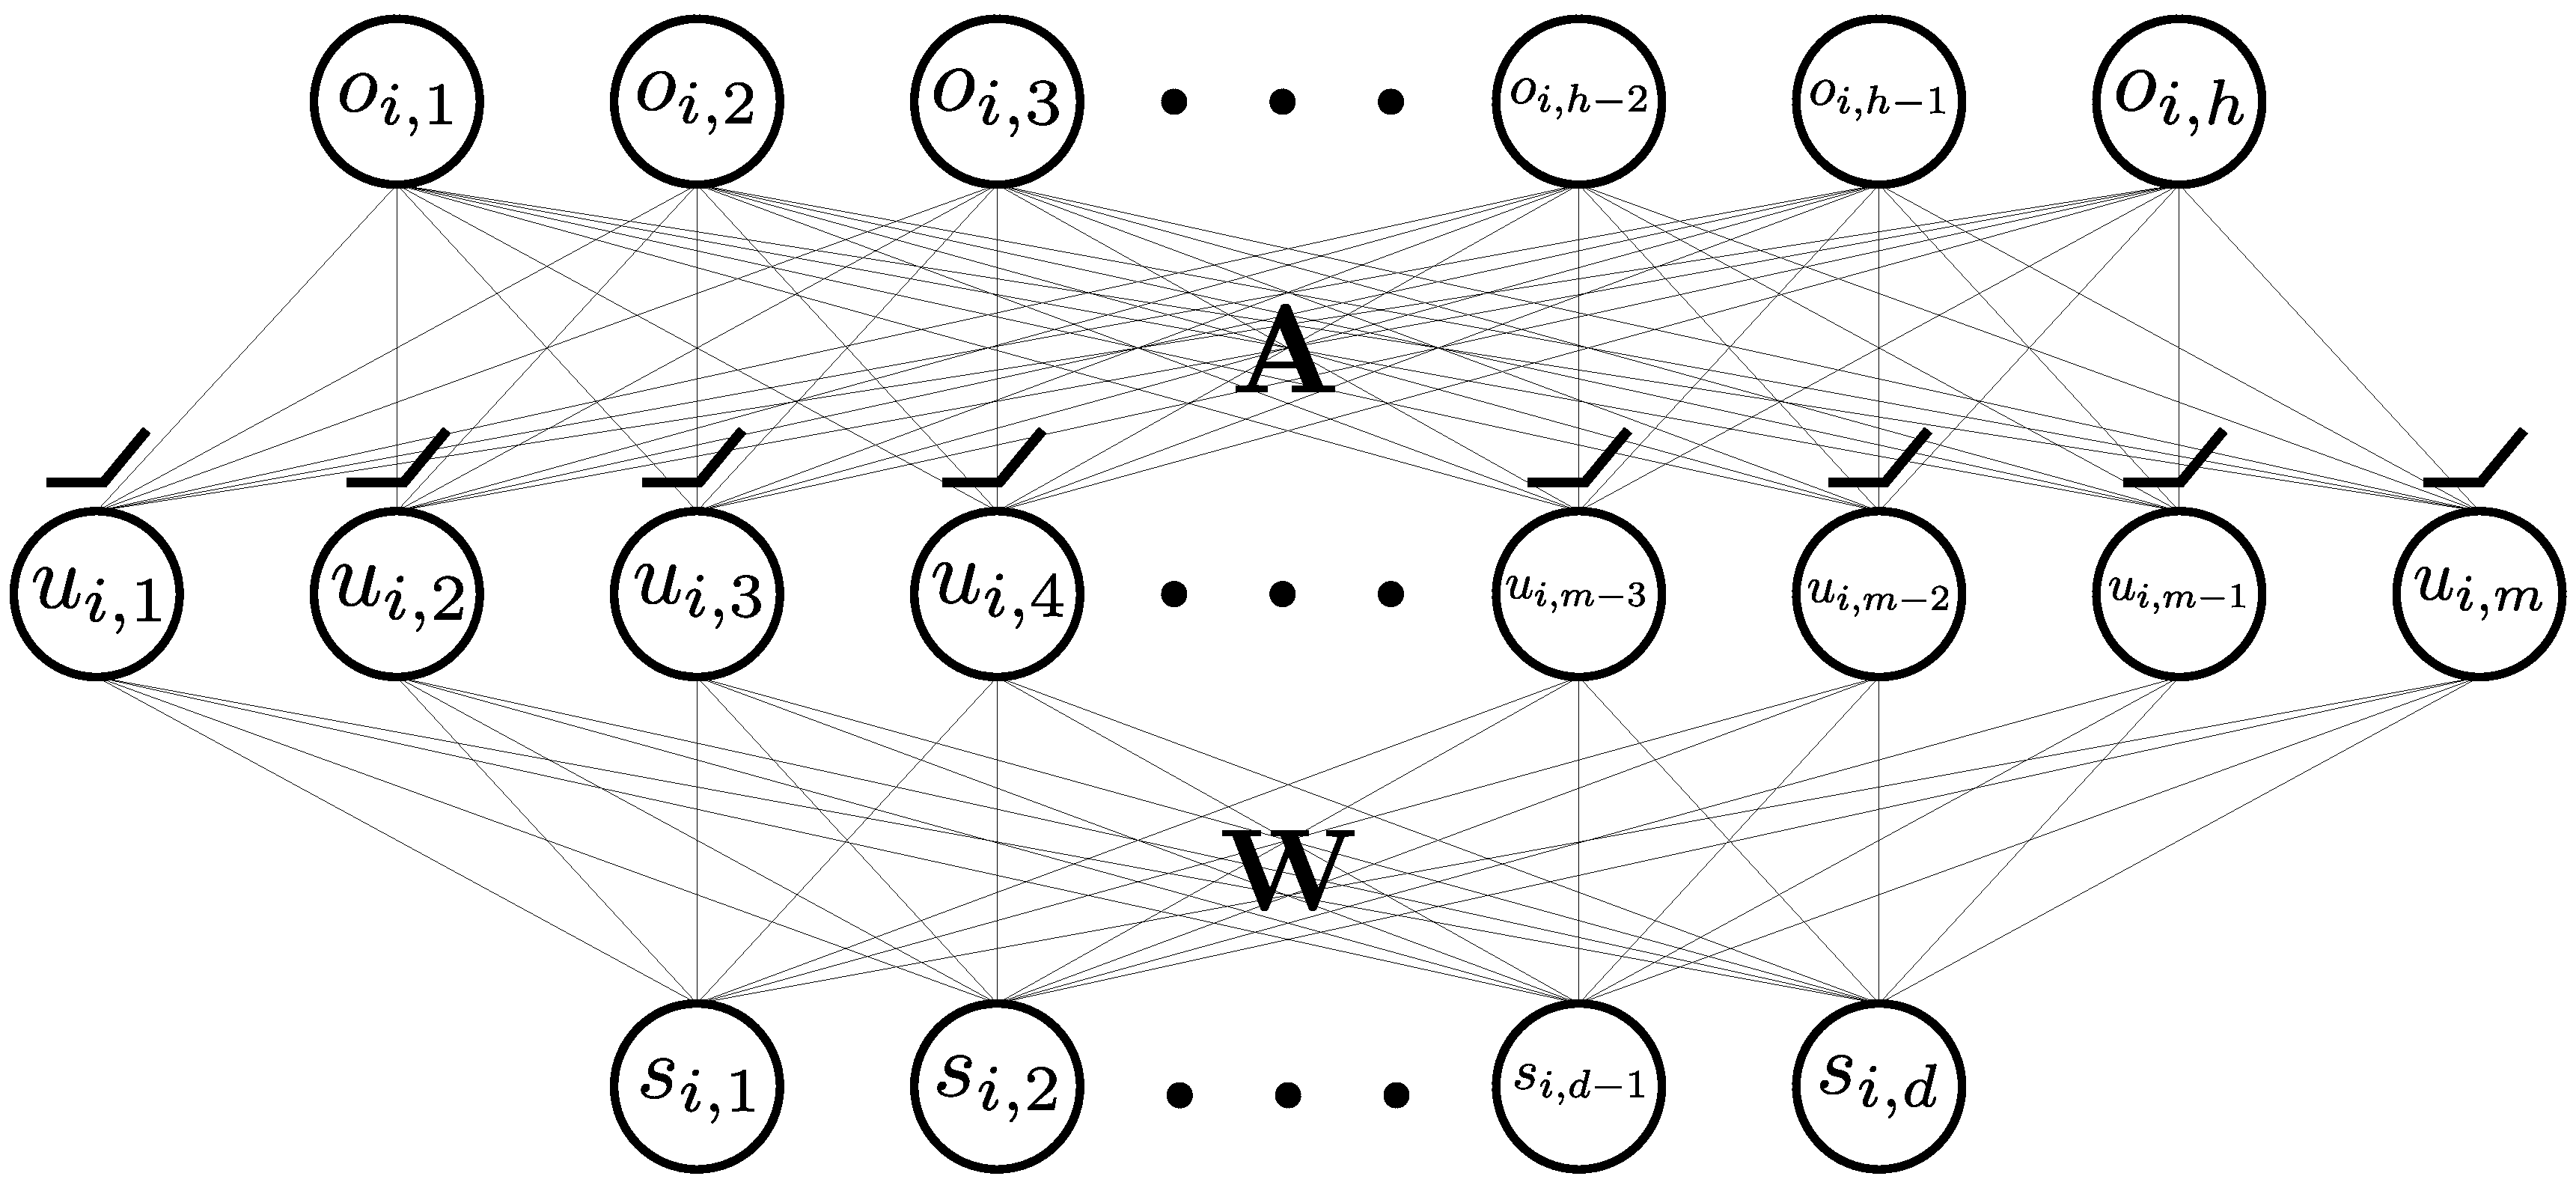
\includegraphics[width=\columnwidth]{nn_value.pdf}}
		\caption{Value neural network.}
		\label{fig:nn_value}
	\end{center}
	\vskip -0.2in
\end{figure}

%The policy neural network defines a family of policies $\rvpi_i \left( \rmW \right)$ parameterized by $\rmW \in \sR^{m \times d}$ given any state $\rvs_i$. Let $\rvpi_i = \rvpi_i \left( \rmW \right)$, the expected loss of the policy neural network can be calculated according to \cref{eq:expected_loss}.

\paragraph{Multi-layered neural networks.} We would like to point that our algorithms and results can be easily extended to general value functions and policies parameterized by multi-layered neural networks \citep{allen2018convergenceA,allen2018convergenceB,du2018gradientA}. For the sake of simplicity and conciseness, we focus on two-layers neural networks in the paper.

%Although there is only one state, i.e., $n = 1$, and $i$ can be omitted without ambiguity, we choose to keep the subscript $i$ here to make the generalization from the standard bandit setting to the many state dependent setting smoother, and our algorithms work for general $n > 1$. For simplicity, we assume $\left\| \rvs_{i} \right\|_2 = 1$, $\forall i \in [n]$.

%In the case of $n > 1$, for each state $\rvs_i$, there is a state dependent policy $\rvpi_i$. And the agent's goal is to learn totally $n$ policies using only one neural network. We assume $\left\| \rvs_{i} -  \rvs_{j} \right\|_2 \ge \delta > 0 , \ \forall i \not= j$, i.e., no duplicated data, and $\left\| \rvs_{i} \right\|_2 = 1, \ \forall i \in [n]$.

\subsection{POLICY GRADIENT}
\label{subsec:policy_gradient}

Our first algorithm follows the widely used policy gradient method. 
Consider at each step $t$, the agent is using $\rvpi\left(\rmW(t)\right)$ as shown in \cref{fig:nn_policy} as its action selection strategy, then the (expected) regret is equivalent to the cumulative expected loss of $\rvpi\left(\rmW(t)\right)$, i.e., 
\begin{equation}
\label{eq:vanilla_policy_gradient_expected_regret}
\begin{split}
    &\sum\limits_{t=0}^{T-1}{{\rvpi^*}^\top \rvr} - \sum\limits_{t=0}^{T-1}{ \expectation\limits_{A_t \sim \rvpi\left(\rmW(t)\right)} \left[ r_{A_t} \right] } \\
    &= \sum\limits_{t=0}^{T-1}{{\rvpi^*}^\top \rvr} - \sum\limits_{t=0}^{T-1}{\rvpi\left(\rmW(t)\right)^\top \rvr},
\end{split}
\end{equation}
by \cref{eq:expected_loss} and \cref{eq:expected_regret}. Using \cref{eq:vanilla_policy_gradient_expected_regret}, at each time step $t$, the agent can use the current NN policy $\rvpi\left(\rmW(t)\right)$ to sample an action, and obtain an estimation of the expected loss $\rvpi\left(\rmW(t)\right)^\top \rvr$. Doing policy gradient updates with respect to the NN weights $\rmW(t)$ will arguably decrease the expected loss, thus reduce the expected regret. 

Unfortunately, the vanilla policy gradient often suffers the ``lack of exploration" problem in practice, i.e., some actions can never be explored thus cannot be learned. Therefore, we propose a two stage algorithm combining policy gradient with uniform exploration as shown in \cref{alg:policy_gradient_uniform_exploration}. After the random initialization, at each step $t$, one of the two cases happens. If $t < T^{\frac{2}{3} + \beta}$, then agent gets into a purely ``exploring phase", without learning the policy neural network, while just collecting empirically estimated rewards. If $t \ge T^{\frac{2}{3} + \beta}$, then the agent starts ``playing and learning". The agent samples and takes actions according to the current neural network policy $\rvpi\left(\rmW(t)\right)$. In the meanwhile, the agent learns the policy neural network by doing policy gradient updates, with the expected empirically estimated loss calculated from the exploring phase as its objective.

\begin{algorithm}[t]
   \caption{Policy Gradient with Uniform Exploration}
\label{alg:policy_gradient_uniform_exploration}
\begin{algorithmic}
   \STATE {\bfseries Input:} State feature $\rvs$, learning rate $\eta > 0$, $\beta > 0$.
   \STATE $\rvw_r(0) \sim \gN\left( 0, \sigma^2 \cdot \rmI \right)$, $\forall r \in [m]$.
   \STATE $a_{k, r} \sim \gU\left\{-1, +1\right\}$, $\forall k \in [h]$, $\forall r \in [m]$.
   \STATE $\hat{r}_{k}\left(0\right) \gets 0$, $n_{k}\left(0\right) \gets 0$, $\forall k \in [h]$.
   \FOR{$t=0$ {\bfseries to} $T-1$}
   \IF{$t < T^{\frac{2}{3} + \beta}$}
   \STATE (Exploring Phase)
   \STATE Uniformly randomly sample action $A_{t} \in [h]$.
   \STATE $\rmW(t+1) \leftarrow \rmW(t)$.
   \ELSE
   \STATE (Playing-Learning Phase)
   \STATE Sample action $A_{t} \sim \rvpi\left(\rmW(t)\right)\left(\cdot \middle| \rvs \right)$.
   \STATE $\rmW(t+1) \leftarrow \rmW(t) + \eta \cdot \frac{d \rvpi\left(\rmW(t)\right)^\top \hat{\rvr} \left(t\right)}{d \rmW(t)}$.
   \ENDIF
   \STATE Take action $A_{t}$. Observe reward $R_{ A_{t}}\left(n_{ A_{t}}\left(t\right) \right)$.
   \STATE $n_{ A_{t}}\left(t+1\right) \gets n_{ A_{t}}\left(t\right) + 1$.
   \STATE $\hat{r}_{A_{t}}\left(t+1\right) \gets \frac{n_{ A_{t}}\left(t\right) \cdot \hat{r}_{A_{t}}\left(t\right) + R_{ A_{t}}\left(n_{A_{t}}\left(t\right)\right) }{n_{ A_{t}}\left(t+1\right)}$.
   \STATE $n_{ k}\left(t+1\right) \gets n_{ k}\left(t\right)$, $\forall k \not= A_t$.
   \STATE $\hat{r}_{k}\left(t+1\right) \gets \hat{r}_{k}\left(t\right)$, $\forall k \not= A_t$.
   \ENDFOR
\end{algorithmic}
\end{algorithm}

\paragraph{Initialization of the matrix $\mathbf{A}$.} Note that in \cref{alg:logit_learning_eps_greedy_exploration} and \cref{alg:policy_gradient_uniform_exploration}, after the random initialization $a_{k,r} \sim \gU\left\{-1, +1\right\}$, $a_{k,r}$ is fixed during learning, which is a common assumption in literature \citep{li2018learning,du2018gradientA,du2018gradientB,allen2018convergenceA,allen2018convergenceB}, and it has been empirically verified that there is no impact on the performance of trained neural networks \citep{hoffer2018fix}. Some other initializations like $\rva_k \sim \gN(0, \rmI)$ also work.

\subsection{LOGIT LEARNING}
\label{subsec:logit_learning}

Our first proposed algorithm is Logit Learning with $\epsilon$-Greedy Exploration, as shown in \cref{alg:logit_learning_eps_greedy_exploration}. After the random initialization, at each time step $t$, the agent selects the action with the largest logit with probability $1 - \epsilon_t$, and it uniformly randomly select actions with the other probability $\epsilon_t$. After taking action and observing rewards, the agent improves its strategies by minimizing the value loss objective $\frac{1}{2} \left\| \rvo\left( \rmW\left(t\right)\right) - \hat{\rvr}\left(t\right) \right\|_2^2$, where $\hat{\rvr}\left(t\right)$ is the empirical mean reward estimated from sampled rewards up to step $t$. In each iteration, the agent only update its value neural network using one gradient descent, therefore the logit learning is in an online fashion.


\begin{algorithm}[t]
	\caption{Logit Learning with $\epsilon$-Greedy Exploration}
	\label{alg:logit_learning_eps_greedy_exploration}
	\begin{algorithmic}
		\STATE {\bfseries Input:} State feature $\rvs$, learning rate $\eta > 0$.
		\STATE $\rvw_r(0) \sim \gN\left( 0, \sigma^2 \cdot \rmI \right)$, $\forall r \in [m]$.
		\STATE $a_{k, r} \sim \gU\left\{-1, +1\right\}$, $\forall k \in [h]$, $\forall r \in [m]$.
		\STATE $\hat{r}_{k}\left(0\right) \gets 0$, $n_{k}\left(0\right) \gets 0$, $\forall k \in [h]$.
		\STATE $\hat{\Delta}_{k}\left(0\right) \gets \max\limits_{k^\prime}\left\{ \hat{r}_{k^\prime}\left(0\right) \right\} - \hat{r}_{k}\left(0\right)$, $\forall k \in [h]$.
		\STATE $\tilde{\Delta}_{k}\left(0\right) \gets \max\limits_{k^\prime}\left\{ o_{k^\prime}\left(0\right) \right\} - o_{k}\left(0\right)$, $\forall k \in [h]$.
		\FOR{$t=0$ {\bfseries to} $T-1$}
		\STATE $\xi_t \gets \frac{\log{t}}{t \hat{\Delta}_{k}^2\left(0\right)}$, $\epsilon_t \gets \min\left\{ \frac{1}{2 h}, \xi_t \right\}$.
		\STATE $\pi_{k}\left(t\right) \gets 1$, for $k = \argmax\limits_{k^\prime \in \left[h\right]}\left\{ o_{ k^\prime}\left(t\right)\right\}$.
		\STATE $\pi_{k}\left(t\right) \gets 0$, $\forall k \not= \argmax\limits_{k^\prime \in \left[h\right]}\left\{ o_{ k^\prime}\left(t\right)\right\}$.
		\STATE $\tilde{\rvpi}\left(t\right) \gets \left( 1 - \epsilon_t \right) \cdot  \rvpi\left(t\right) + \epsilon_t \cdot \gU{\left[ h \right]}$.
		\STATE Sample action $A_{t} \sim \tilde{\rvpi}\left(t\right)\left(\cdot \middle| \rvs \right)$.
		\STATE Take action $A_{t}$. Observe reward $R_{ A_{t}}\left(n_{ A_{t}}\left(t\right) \right)$.
		\STATE $n_{A_{t}}\left(t+1\right) \gets n_{ A_{t}}\left(t\right) + 1$.
		\STATE $\hat{r}_{A_{t}}\left(t+1\right) \gets \frac{n_{ A_{t}}\left(t\right) \cdot \hat{r}_{A_{t}}\left(t\right) + R_{A_{t}}\left(n_{A_{t}}\left(t\right)\right) }{n_{ A_{t}}\left(t+1\right)}$.
		\STATE $n_{k}\left(t+1\right) \gets n_{ k}\left(t\right)$, $\forall k \not= A_t$.
		\STATE $\hat{r}_{k}\left(t+1\right) \gets \hat{r}_{k}\left(t\right)$, $\forall k \not= A_t$.
		\STATE $\rmW(t+1) \leftarrow \rmW(t) - \eta \cdot \frac{d \left\{ \frac{1}{2} \left\| \rvo\left( \rmW\left(t\right)\right) - \hat{\rvr}\left(t\right) \right\|_2^2 \right\}}{d \rmW(t)}$.
		\ENDFOR
	\end{algorithmic}
\end{algorithm}